%!TEX root=../root.tex

%%%%%%%%%%%%%%%%%%%%%%%%%%%%%%%%%%%%%%%%%%%%%%%%%%%%%%%%%%%%%%%%%%%%%%%%%%%%%%%%
%2345678901234567890123456789012345678901234567890123456789012345678901234567890
%        1         2         3         4         5         6         7        
\section{TRAJECTORY-DEPENDENT ERROR SYSTEM}
In this section, we introduce the transformation of the underwater dynamic model into an error system when the robot tracks a trim trajectory. Moreover, the linearization of the error dynamics is discussed.
 
\subsection{Frenet-Serret Frame}
When the robot moves along a smooth curve $\vec{r}(t)=(x(t)~y(t)~z(t))^{T}$ in the three-dimensional Euclidean space $\mathbb{R}^{3}$, its motion can be characterized by three unit vectors: $T^{i}(t)$, $N^{i}(t)$ and $B^{i}(t)$. $T^{i}(t)$ is a unit vector tangent to the curve denoting the motion direction, which can be calculated as the changing rate of the curve vector with respect to its arclength $s$:
\begin{equation}
T^{i}(t)=\dfrac{d\vec{r}}{ds}=\frac{\vec{r}^{'}(t)}{||\vec{r}^{'}(t)||}.
\end{equation}
The normal vector $N^{i}(t)$ is defined as the derivative of $T^{i}$  with respect to the arclength $s$ of the curve, divided by its length:
\begin{equation}
N^{i}(t)=\dfrac{\dfrac{dT^{i}(t)}{ds}}{\left|\left|\dfrac{dT^{i}(t)}{ds}\right|\right|}=\dfrac{(T^{i})^{'}(t)}{||(T^{i})^{'}(t)||}=\dfrac{\vec{r}^{'}(t)\times (\vec{r}^{''}(t)\times \vec{r}^{'}(t))}{||\vec{r}^{'}(t)||~||\vec{r}^{''}(t)\times \vec{r}^{'}(t)||}.
\end{equation}
The binormal vector $B^{i}_{T}$ is the cross product of the normal vector $N^{i}(t)$ and the tangent vector $T^{i}(t)$ and is calculated as 
\begin{equation}
B^{i}(t)=T^{i}(t)\times N^{i}(t)=\frac{\vec{r}^{''}(t)\times \vec{r}^{'}(t)}{||\vec{r}^{''}(t)\times \vec{r}^{'}(t)||}.
\end{equation}
\subsection{Trim Trajectory}
The concept of trim trajectories originates in the path planning for aircrafts. It corresponds to a curve $\vec{p}_{\mathcal{T}}=(x_{\mathcal{T}}~y_{\mathcal{T}}~z_{\mathcal{T}})^{T}
\in \mathbb{R}^{3}$ that the robot can follow in a steady-state equilibrium. A trim trajectory $\vec{p}_{\mathcal{T}}$ is parametrized by three parameters $\vec{p}_{\mathcal{T}}: (||\vec{v}_{\mathcal{T}}||~\dot{\phi}_{\mathcal{T}}~\gamma_{T})^{T}$, where $\vec{v}_{\mathcal{T}}$ is the trim speed. We choose the aforementioned Frenet-Serret frame as the desired body frame for the robot moving along the trim trajectory curve and denote it as $\lbrace \mathcal{T} \rbrace$. The desired orientation on basis of $\lbrace \mathcal{T} \rbrace$ for the trim trajectory is represented as $\vec{\eta}_{\mathcal{T}}=(\phi_{\mathcal{T}}~\theta_{\mathcal{T}}~\psi_{\mathcal{T}})^{T}$. For $\lbrace \mathcal{T} \rbrace$, the trim speed is equal to the desired surge velocity $u$. The angle $\gamma_{\mathcal{T}}$ is the flight path angle. The trim yaw angle is given by $\phi_{\mathcal{T}}(t)=\dot{\phi}_{\mathcal{T}}t+\phi_{0}$, where $\dot{\phi}_{\mathcal{T}}\in \mathbb{R}$ is the constant yaw rate and $\phi_{0}\in [0,2\pi)$ is the initial yaw angle. Along the trim trajectory, the roll and pitch angle remain unchanged, i.e., $\dot{\phi}_{\mathcal{T}}=0$ and $\dot{\theta}_{\mathcal{T}}=0$. 
\begin{figure}[thpb]
\centering
\includegraphics[width=2.5in]{trimtraj.eps}
\caption{Trim trajectory}
\label{FinGeo}
\end{figure} 
A trim trajectory segment corresponds to a helix with radius $||\vec{v}_{\mathcal{T}}||\dot{\psi}_{\mathcal{T}}^{-1}\cos(\gamma_{\mathcal{T}})$ and is represented as
\begin{align}
&\vec{p}_{\mathcal{T}}(t)= \nonumber
\\&||\vec{v}_{\mathcal{T}}||\dot{\psi}_{\mathcal{T}}^{-1}\cos(\gamma_{\mathcal{T}})
\begin{bmatrix}
\sin(\psi_{\mathcal{T}}(t)-\psi_{v})-\sin(\psi_{0}-\psi_{v}) \\
\cos(\psi_{\mathcal{T}}(t)-\psi_{v})+\cos(\psi_{0}-\psi_{v}) \\
-\dot{\psi}_{\mathcal{T}}\tan(\gamma_{\mathcal{T}})t
\end{bmatrix}+
\vec{p}_{0},\label{EQ:pT}
\end{align}
where $\vec{p}_{0}=(x_{0}~y_{0}~z_{0})^{T} \in \mathbb{R}^{3}$ is the initial trim position.
The transformation matrix from the Frenet-Serret frame $\lbrace \mathcal{T} \rbrace$ to the inertial world frame $\lbrace i \rbrace$ is defined as $
 \mathcal{R}_{\mathcal{T}}:=
 (T^{i}(t)~N^{i}(t)~B^{i}(t))$. The desired trim roll and pitch angle can be inferred from the Frenet-Serret frame setting as $\theta_{\mathcal{T}}=-\sin^{-1}(\vec{T}^{i}(t))$ and $
\phi_{\mathcal{T}}=-\sin^{-1}(\sec(\theta_{\mathcal{T}})\cdot \vec{N}^{i}(t))
$, respectively. Stacking the two dynamic-affecting angles together we define $\vec{\eta}_{p,\mathcal{T}}=(\phi_{\mathcal{T}}~\theta_{\mathcal{T}})^{T}$. With the value of $\phi_{\mathcal{T}}$ and $\theta_{\mathcal{T}}$, we can obtain the angular velocity transformation matrix $\mathcal{Q}_{\mathcal{T}}$. Thus, the desired velocities along the trim trajectory can be calculated as
\begin{equation}
\begin{bmatrix}
\vec{v}_{\mathcal{T}} \\
\vec{w}_{\mathcal{T}}
\end{bmatrix} =
\begin{bmatrix}
\mathcal{R}_{\mathcal{T}}^{-1} & 0\\
0 & \mathcal{Q}_{\mathcal{T}}^{-1} 
\end{bmatrix}
\begin{bmatrix}
\vec{p}_{\mathcal{T}} \\ \vec{\eta}_{\mathcal{T}}
\end{bmatrix}.
\end{equation}
All the variables affecting the underwater robot dynamics ($\vec{v}_{\mathcal{T}}$, $\vec{w}_{\mathcal{T}}$, $\vec{\eta}_{p,\mathcal{T}}$), see~(\ref{EQ:RobotDynamics}), stay constant. They correspond to the equilibrium point for motion along the trim trajectory. The equilibrium input corresponding to $\dot{\vec{v}}_{\mathcal{T}}=\vec{0}$ and $\dot{\vec{w}}_{\mathcal{T}}=\vec{0}$ can be calculated as
\begin{align}
\vec{\tau}_{d,\mathcal{T}}=&C_{RB}(\vec{x}_{dyn,\mathcal{T}},\vec{r}_{T},\mathfrak{d}_{H},\mathfrak{d}_{F})
\begin{bmatrix}
\vec{v}_{\mathcal{T}} \\ \vec{w}_{\mathcal{T}}
\end{bmatrix}
+ 
C_{A}(\vec{x}_{dyn,\mathcal{T}},\mathfrak{d}_{H})\vec{\upsilon}_{\mathcal{T}}+ \nonumber \\ & D(\vec{x}_{dyn,\mathcal{T}},\mathfrak{d}_{H})\vec{\upsilon}_{\mathcal{T}} 
+\vec{g}(\vec{x}_{kin,\mathcal{T}},\mathfrak{d}_{F},\vec{r}_{T},\mathfrak{d}_{H}).
\end{align}
The underwater dynamics can be linearized for explicit values of $\vec{v}_{\mathcal{T}}, \vec{w}_{\mathcal{T}}$, $\vec{\eta}_{p,\mathcal{T}}$ and $\vec{u}_{\mathcal{T}}$. 
The state space form of the underwater robotic system is given by
\begin{equation}
\frac{d}{dt}\begin{bmatrix}
\vec{x}_{dyn} \\
\vec{x}_{kin}
\end{bmatrix}=
\begin{bmatrix}
\vec{f}_{dyn}(\vec{x}_{dyn},\vec{x}_{kin}) \\
\vec{f}_{kin}(\vec{x}_{dyn},\vec{x}_{kin})
\end{bmatrix} +
\begin{bmatrix}
\vec{g}_{dyn}(\vec{x}_{dyn},\vec{u}) \\
\vec{0}
\end{bmatrix}.
\end{equation}
Equivalently, they can be written in the following form:
\begin{empheq}[left=\empheqlbrace]{align}
& \frac{d}{dt}\vec{v}=\vec{f}_{\vec{v}}(\vec{v},\vec{w})+\vec{f}_{\vec{v}}^{\vec{\eta}}(\vec{\eta}_{p})+\vec{g}_{\vec{v}}
(\vec{v},\vec{u}) \label{EQ:SS_v} \\
&\frac{d}{dt}\vec{w}=\vec{f}_{\vec{w}}(\vec{v},\vec{w})+
\vec{f}_{\vec{w}}^{\vec{\eta}}(\vec{\eta}_{p})+
\vec{g}_{\vec{w}}
(\vec{v},\vec{u}) \label{EQ:SS_w} \\
& \frac{d}{dt}\vec{p} =\mathcal{R}(\vec{\eta})\vec{v}  \\
&\frac{d}{dt}\vec{\eta}=\mathcal{Q}(\vec{\eta}_{p})\vec{\omega}.
\end{empheq}
where $\vec{\eta}_{p}=(\phi~\theta)^{T}$ denotes the partial kinematic states affecting the underwater robot dynamics appearing in the restoring term $\vec{g}(\vec{\eta})$, $\mathcal{R}$ is the linear velocity transformation matrix from $\lbrace b \rbrace$ to $\lbrace i \rbrace$ and $\mathcal{Q}$ is the transformation matrix  relating the body fixed angular velocity $\vec{w}$ to Euler angle rates. We now need to convert (\ref{EQ:RobotDynamics}) into the state space form, see (\ref{EQ:SS_v}) and (\ref{EQ:SS_w}).  

The first three rows of the matrix $B_{a}$ are denoted by $B_{a,f}\in \mathbb{R}^{3\times(n_{t}+n_{f})}$ and the last three rows of the matrix are represented by $B_{a,m}\in \mathbb{R}^{3\times(n_{t}+n_{f})}$. The generalized force generated by the actuators can be represented as $\vec{\tau}=B_{a}\vec{u}$. Separately written, $\vec{f}=\emph{\textbf{B}}_{a,f}\vec{u}$ and $\vec{m}=\emph{\textbf{B}}_{a,m}\vec{u}$, where $\vec{f}$ is the force vector along the $x_b$-, $y_b$- and $z_b$-axes of $\lbrace b \rbrace$ and $\vec{m}$ is the moment vector about  those axes. Hence, for our modeling approach, we get $\vec{g}_{\vec{v}}(\vec{v},\vec{u})=M^{-1}B_{a,f}\vec{u}$ and
$\vec{g}_{\vec{w}}(\vec{v},\vec{u})=M^{-1}B_{a,m}\vec{u}$. The rigid body Coriolis-centripetal matrix $C_{RB}(\vec{v},\vec{w})$ can be separated into $C_{RB,\vec{v}}$ and $C_{RB,\vec{w}}$ corresponding to the first and last three rows of the Coriolis matrix $C_{RB}$, respectively. Similarly, we assign the first three lines of the added mass Coriolis matrix $C_{A}$ to $C_{A,\vec{v}}(\vec{v},\vec{w})$ and the last three lines to $C_{A,\vec{w}}(\vec{v},\vec{w})$. 
%\begin{equation}
%\emph{\textbf{C}}_{A,\vec{w}}(\vec{v},\vec{w})=
%\begin{bmatrix}
%0&-Z_{\dot{w}}w&Y_{\dot{v}}v&0&-N_{\dot{r}}\dot{r}&M_{\dot{q}}q\\
%Z_{\dot{w}}w&0&-X_{\dot{u}}u&N_{\dot{r}}r&0&-K_{\dot{p}}p\\
%-Y_{\dot{v}}v&X_{\dot{u}}u&0&-M_{\dot{q}}q&K_{\dot{p}}p&0
%\end{bmatrix}
%\end{equation}
The restoring vector $\vec{g}(\vec{\eta})$ can also be separated in the same way into $\vec{g}_{\vec{v}}(\vec{\eta})\in \mathbb{R}^{3}$ that is the first three elements of $\vec{g}(\vec{\eta})$ and $\vec{g}_{\vec{w}}(\vec{\eta})\in \mathbb{R}^{3}$ corresponding to the last three elements. 
To sum up, we can obtain the following relationship between the terms in the underwater robot dynamics and the state-space terms:
\begin{align}
\vec{f}_{\vec{v}}(\vec{v},\vec{w})&=-M^{-1}(C_{RB,\vec{v}}+C_{A,\vec{v}}+D_{\vec{v}}), \label{EQ:fv}\\
\vec{f}_{\vec{w}}(\vec{v},\vec{w})&=-M^{-1}(C_{RB,\vec{w}}+C_{A,\vec{w}}+D_{\vec{w}}), \label{EQ:fw} \\
\vec{f}_{\vec{v}}^{\vec{\eta}}(\vec{\eta}_{p})&=-M^{-1}\vec{g}_{\vec{v}}(\vec{\eta}), \label{EQ:fveta}\\
\vec{f}_{\vec{w}}^{\vec{\eta}}(\vec{\eta}_{p})&=-M^{-1}\vec{g}_{\vec{w}}(\vec{\eta})\label{EQ:fweta}.
\end{align}
%\begin{figure*}[!t]
% ensure that we have normalsize text
%\normalsize
% Store the current equation number.
%\setcounter{mytempeqncnt}{\value{equation}}
% Set the equation number to one less than the one
% desired for the first equation here.
% The value here will have to changed if equations
% are added or removed prior to the place these
% equations are referenced in the main text.
%\setcounter{equation}{5}
%\begin{equation}
%\label{eqn_dbl_x}
%\emph{\textbf{C}}_{RB,\vec{v}}= \\
%\begin{bmatrix}
%0&0&0&m(y_{g}q+z_{g}r)&-m(x_{g}q-w)&-m(x_{g}r+v)\\
%0&0&0&-m(y_{g}p+w)&m(z_{g}r+x_{g}p)&-m(y_{g}r-u)\\
%0&0&0&-m(z_{g}p-v)&-m(z_{g}q+u)&m(x_{g}p+y_{g}q)\\
%\end{bmatrix} 
%\end{equation}
%\begin{gather}\label{EQ:CoriolisRigidBodyW}
%\emph{\textbf{C}}_{RB,\vec{\omega}}(\vec{v},\vec{\omega})=
%\left[
%\begin{matrix} -m(y_{g}+z_{g}r)&m(y_{g}p+w)&m(z_{g}p-v)\\
%m(x_{g}q-w)&-m(z_{g}r+x_{g}p)&m(z_{g}q+u)\\
%m(x_{g}r+v)&m(y_{g}r-u)&-m(x_{g}p+y_{g}q)
%\end{matrix}
%\right.
% \nonumber\\
%\qquad \qquad\left. \begin{matrix} 
%0 & -I_{yz}q-I_{xz}p+I_{z}r & I_{yz}r+I_{xy}p-I_{y}q \\
%I_{yz}q+I_{xz}p-I_{z}r &0& -I_{xz}r-I_{xy}q+I_{x}p \\
%-I_{yz}r-I_{xy}p+I_{y}q&I_{xz}r+I_{xy}q-I_{x}p &0  \end{matrix}
%\right]
%\end{gather}
%\begin{equation}
%\vec{g}_{\vec{v}}(\vec{\eta})=
%\begin{bmatrix}
%(W-B)\sin(\theta)\\
%-(W-B)\cos(\theta)\sin(\phi)\\
%-(W-B)\cos(\theta)\cos(\phi)
%\end{bmatrix}\label{EQ:RstV}
%\end{equation}
%\begin{equation}
%\vec{g}_{\vec{\omega}}(\vec{\eta})=
%\begin{bmatrix}
%-(y_{g}W-y_{b}B)\cos(\theta)\cos(\phi)+(z_{g}W-%z_{b}B)\cos(\theta)\sin(\phi)\\
%(z_{g}W-z_{b}B)\sin(\theta)+(x_{g}W-x_{b}B)\cos(\theta)\cos(\phi)\\
%-(x_{g}W-x_{b}B)\sin(\theta)\cos(\phi)-(y_{g}W-y_{b}B)\sin(\theta)
%\end{bmatrix}\label{EQ:RstW}
%\end{equation}
% Restore the current equation number.
%\setcounter{equation}{\value{mytempeqncnt}}
% IEEE uses as a separator
%\hrulefill
% The spacer can be tweaked to stop underfull vboxes.
%\vspace*{4pt}
%\end{figure*}
\subsection{Nonlinear Transformation and Error Dynamics}
Fig.~\ref{FIG:FrameRelationship} shows the relationship between the inertial world frame $\lbrace i \rbrace$, the robot body frame $\lbrace b \rbrace$ and the Frenet-Serret frame along the trim curve $\lbrace \mathcal{T} \rbrace$. In the ideal case, the robot body frame $\lbrace b \rbrace$ should coincide with the frame $\lbrace \mathcal{T} \rbrace$ for perfect tracking, but it is not necessarily the case in reality. Therefore, we use $\mathcal{R}_{E}$ to denote  the transformation matrix from $\lbrace b \rbrace$ to $\lbrace \mathcal{T} \rbrace$ for linear velocities and position and $\mathcal{Q}_{E}$ for angular velocities. Based on these definitions, we have the following relationship $\mathcal{R}_{E}=\mathcal{R}_{\mathcal{T}}^{-1}\mathcal{R}$ and $\mathcal{Q}_{E}=\mathcal{Q}_{\mathcal{T}}^{-1}\mathcal{Q}$. We adopt the following transformation for the state errors: $\vec{v}_{E}=\vec{v}-\vec{v}_{\mathcal{T}}$, $\vec{w}_{E}=\vec{w}-\vec{w}_{\mathcal{T}}$, $\vec{p}_{E}=\mathcal{R}^{-1}(\vec{p}-\vec{p}_{\mathcal{T}})$ and $\vec{\eta}_{E}=\mathcal{R}^{-1}(\vec{\eta}-\vec{\eta}_{\mathcal{T}})$, which can be interpreted as the errors 
between the desired trim states and the real robot states as measured by sensors in the robot body frame $\lbrace b \rbrace$. We define the error dynamics input as $\vec{u}_{E}=\vec{u}-\vec{u}_{\mathcal{T}}$, where $\vec{u}$ is the control input from the actuators and $\vec{u}_{\mathcal{T}}$ is the desired trim actuator input, which is calculated as $\vec{u}_{\mathcal{T}}=B_{a}^{-1}\vec{\tau}_{d,\mathcal{T}}$.
\begin{figure}[thpb]
\center
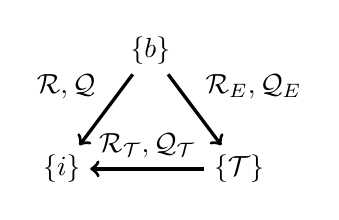
\begin{tikzpicture}[scale=0.75]
\node (A) at (0,0){$\lbrace i \rbrace$};
\node (B) at (1.5,2){$\lbrace b \rbrace$};
\node (C) at (3,0){$\lbrace \mathcal{T} \rbrace$};
\draw[->, very thick] (B) to
node[above left] {$\mathcal{R}, \mathcal{Q}$} (A);
\draw[->, very thick] (C) to
node[above] {$\mathcal{R}_{\mathcal{T}}, \mathcal{Q}_{\mathcal{T}}$} (A);
\draw[->, very thick] (B) to
node[above right] {$\mathcal{R}_{E}, \mathcal{Q}_{E}$} (C);
\end{tikzpicture}
\caption{Frame relationship}	
\label{FIG:FrameRelationship}
\end{figure}

\subsection{Linearization of Error System}
In the previous section, we have derived the equilibrium point for the motion of the \ac{auv} along a trim trajectory and defined the error system for tracking this trajectory. It is common to control a nonlinear system by linearizing it at an equilibrium point. Moreover, we can use properties of the linearized system as performance criteria for finding an optimal geometry, e.g., the controllability matrix. Thus, in this section, we perform the linearization of (\ref{EQ:fv}), (\ref{EQ:fw}), (\ref{EQ:fveta}) and (\ref{EQ:fweta}) at ($\vec{v}_{\mathcal{T}}$, $\vec{w}_{\mathcal{T}}$, $\vec{\eta}_{p,\mathcal{T}}$, $\vec{u}_{\mathcal{T}}$),

\begin{empheq}[left=\empheqlbrace]{align}
&\dfrac{d}{dt}\delta\vec{v}_{E}=A_{\vec{v}}^{\vec{v}}
\delta\vec{v}_{E}+A_{\vec{v}}^{\vec{\omega}}
\delta\vec{\omega}_{E}+A_{\vec{v}}^{\vec{\eta}}
\delta\vec{\vec{\eta}}_{E}+B_{\vec{v}}\delta\vec{u} \\
&\dfrac{d}{dt}\delta\vec{w}_{E}=A_{\vec{w}}^{\vec{v}}
\delta\vec{v}_{E}+A_{\vec{w}}^{\vec{w}}
\delta\vec{w}_{E}+A_{\vec{w}}^{\vec{\eta}}
\delta\vec{p}_{E}+B_{\vec{w}}\delta\vec{u} 
\end{empheq} 
where
\begin{empheq}[left=\empheqlbrace]{align}
&A_{\vec{v}}^{\vec{v}}=\dfrac{\partial}{\partial \vec{v}}[\vec{f}_{\vec{v}}(\vec{v},\vec{w})+\vec{g}_{\vec{v}}(\vec{v},\vec{w},\vec{u})]
 \\
&A_{\vec{v}}^{\vec{w}}=\dfrac{\partial}{\partial \vec{w}}[\vec{f}_{\vec{v}}(\vec{v},\vec{w})+\vec{g}_{\vec{v}}(\vec{v},\vec{w},\vec{u})]
\\
&A_{\vec{v}}^{\vec{\eta}}=\dfrac{\partial}{\partial \vec{\eta}}\vec{f}_{\vec{v}}^{\vec{\eta}}(\vec{\eta}_{p})\\
&B_{\vec{v}}=\dfrac{\partial}{\partial \vec{u}}
\vec{g}_{\vec{v}}(\vec{v},\vec{w},\vec{u})
\end{empheq} 
and
\begin{empheq}[left=\empheqlbrace]{align}
&A_{\vec{w}}^{\vec{v}}=\dfrac{\partial}{\partial \vec{v}}[\vec{f}_{\vec{w}}(\vec{v},\vec{w})+\vec{g}_{\vec{w}}(\vec{v},\vec{w},\vec{u})]
 \\
&A_{\vec{w}}^{\vec{w}}=\dfrac{\partial}{\partial \vec{w}}[\vec{f}_{\vec{w}}(\vec{v},\vec{w})+\vec{g}_{\vec{v}}(\vec{v},\vec{w},\vec{u})]
\\
&A_{\vec{w}}^{\vec{\eta}}=\dfrac{\partial}{\partial \vec{\eta}}\vec{f}_{\vec{w}}^{\vec{\eta}}(\vec{\eta}_{p})\\
&B_{\vec{w}}=\dfrac{\partial}{\partial \vec{u}}
\vec{g}_{\vec{w}}(\vec{v},\vec{w},\vec{u}).
\end{empheq} 
The calculation of linearizing the position and Euler angle error can be found in~\cite{c4}. The resulting linearization is 
\begin{empheq}[left=\empheqlbrace]{align}
&\dfrac{d}{dt}\delta\vec{p}_{E}=\delta \vec{v}_{E}-\mathcal{S}(\vec{w}_{\mathcal{T}})\delta \vec{p}_{E}-\mathcal{S}(\vec{v}_{\mathcal{T}})\delta \vec{\eta}_{E} \\
&\dfrac{d}{dt}\delta\vec{\eta}_{E}=\delta \vec{w}_{E}- \mathcal{S}(\vec{w}_{\mathcal{T}}) \delta \vec{\eta}_{E},
\end{empheq} 
where $\mathcal{S}$ is a skew-symmetrical matrix satisfying $\mathcal{S}=\mathcal{S}^{T}$ and defined as
\begin{equation}
\mathcal{S}(\vec{\zeta})=-\mathcal{S}^{T}(\vec{\zeta})=
\begin{bmatrix}
0&-\zeta_{3}&\zeta_{2}\\
\zeta_{3}&0&-\zeta_{1}\\
-\zeta_{2}&\zeta_{1}&0
\end{bmatrix}
\end{equation}
for an arbitrary vector $\vec{\zeta}=(\zeta_{1}~\zeta_{2}~\zeta_{3})^{T}$. 
In total, the linearized error dynamics are 
\begin{empheq}[left=\empheqlbrace]{align}
&\dfrac{d}{dt}\delta\vec{x}_{dyn_{E}}=A_{d}^{d}\delta\vec{x}_{dyn_{E}}+
A_{k}^{d}\delta\vec{x}_{kin_{E}}+B\vec{u} \\
&\dfrac{d}{dt}\delta\vec{x}_{kin_{E}}=\delta\vec{x}_{dyn_{E}}+A_{k}^{k}
\delta\vec{x}_{kin_{E}}
\end{empheq}
where $\delta\vec{x}_{dyn_{E}}=(\delta\vec{v}_{E}~\delta\vec{\omega}_{E})^{T}\in \mathbb{R}^{6}$ denotes the 6 dynamic error states (velocity errors) and
$\delta\vec{x}_{kin_{E}}=(\delta \vec{p}_{E}~\delta \vec{\lambda}_{E})^{T}\in \mathbb{R}^{6}$ are the 6-dimensional kinematic states. 
The error dynamics system matrices $A_{d}^{d}$ and $A_{k}^{d}$ are defined as 
\begin{align}
A_{d}^{d}=
\begin{bmatrix}
A_{\vec{v}}^{\vec{v}}&A_{\vec{v}}^{\vec{\omega}}\\
A_{\vec{\omega}}^{\vec{v}}&A_{\vec{\omega}}^{\vec{\omega}}
\end{bmatrix}\in \mathbb{R}^{6 \times 6}, \quad
A_{k}^{d}=
\begin{bmatrix}
0&A_{\vec{v}}^{\vec{\eta}}\\
0&A_{\vec{\omega}}^{\vec{\eta}}
\end{bmatrix} \in \mathbb{R}^{6 \times 6},
\end{align}
respectively. The matrix $A_{d}^{d}$ indicates the mutual interaction between the linear velocities and angular velocities, while the matrix $A_{k}^{d}$ represents the influence of the kinematic states on the dynamic states.
The kinematic error system matrix $A_{k}^{k}$ is defined as   
\begin{align}
A_{k}^{k}=
\begin{bmatrix}
-\mathcal{S}(\vec{\omega}_{\mathcal{T}})&-\mathcal{S}(\vec{v}_{\mathcal{T}})\\
0&-\mathcal{S}(\vec{\omega}_{\mathcal{T}})
\end{bmatrix}\in \mathbb{R}^{6 \times 6}.
\end{align}
The input matrix is given as $B=(B_{\vec{v}}~B_{\vec{\omega}})^{T} \in \mathbb{R}^{(n_{t}+n_{f})\times 6}$.
From the previous analysis, we come to the conclusion that the linearized error dynamic system, see Fig.~\ref{ErrorSystem}, is a bijective function of trim trajectories $\vec{p}_{\mathcal{T}}:(||\vec{v}_{\mathcal{T}}||,   \dot{\psi}_{\mathcal{T}}, \gamma_{\mathcal{T}})^{T}$. This property is of significance, since we can adopt the methods for \ac{mimo} linear systems to handle the originally nonlinear and strongly coupled system. 
\setlength{\arraycolsep}{5pt}
\begin{figure}
\centering
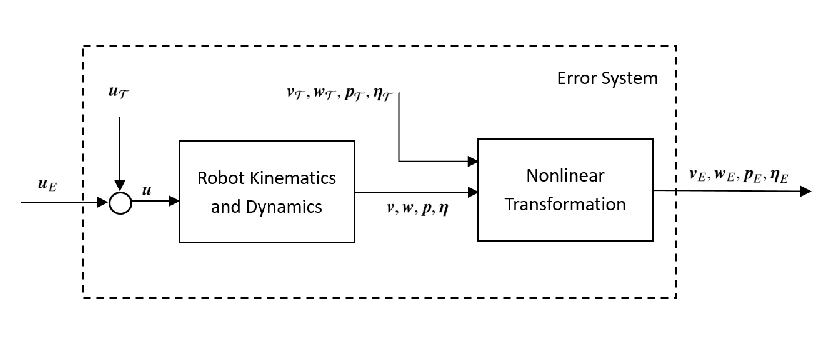
\includegraphics[width=3in]{errordynamics.eps}
\caption{Error System}
\label{ErrorSystem}
\end{figure}
Suppose the robot should track $m$ trim trajectories, which can be combined as \emph{motion primitives} to form a complex path. By implementing the aforementioned nonlinear transformation and linearizing at the trim equilibrium points, we will obtain $m$ linearized error dynamic systems 
\begin{equation}
 	\dot{\vec{x}}_{E,j}=A_{E,j}\vec{x}_{E,1}+B_{E,j}\vec{u}_{E,j}, \quad \text{for} \,\, j=1, \cdots, m, j
 \end{equation} 
 representing the index for the trim trajectory, where $\vec{x}_{E,j}=(\vec{v}_{E,j}~\vec{w}_{E,j}~\vec{p}_{E,j}~\vec{\eta}_{E,j})^{T}$, the error dynamics system matrix
\begin{equation}
A_{E,j}=
\begin{bmatrix}
A_{d,j}^{d}&A_{k,j}^{d}\\
I_{6 \times 6}&A_{d,j}^{d}
\end{bmatrix} \in \mathbb{R}^{12 \times 12}
\end{equation}
and the error dynamics input matrix 
\begin{equation}
B_{E,j}=
\begin{bmatrix}
B_{\vec{v},j} \\
B_{\vec{w},j} 
\end{bmatrix} \in \mathbb{R}^{12 \times (n_{t}+n_{f})}.
\end{equation}
For the complete trim path, we can formulate the error system along the $m$ trim trajectories as a switched system
\begin{align}
\Sigma_{S,A_{E},B_{E}}: \dot{\vec{x}}_{E}(t)=
A_{E}(t)\vec{x}_{E}(t)+B_{E}(t)\vec{u}_{E}(t),
\end{align}
where $A_{E}(t)\in\lbrace A_{E,1}, \cdots, A_{E,m}\rbrace$ and $B_{E}(t)\in\lbrace B_{E,1}, \cdots, B_{E,m}\rbrace$.
\subsection{Switched \ac{lqr}}
For each linearized trim segment, we design a \acl{lqr}  with weighting matrix $ \mathcal{Q}_{E,j}$ and $\mathcal{R}_{E,j}$, for $j=1, \cdots, m$, to minimize the cost function for the $j$-th trim trajectory
\begin{align}
J=\int^{\infty}_{0}[\vec{x}_{E,j}^{T}\mathcal{Q}_{E,j}\vec{x}_{E,j}+\vec{u}_{E,j}^{T}\mathcal{R}_{E,j}
\vec{u}_{E,j}]dt
\end{align}
subject to $\vec{x}_{E,j}(0)=\vec{x}_{E,j,0}$, $\mathcal{Q}_{E,j} \succeq 0$, $\mathcal{Q}_{E,j}^{T}=\mathcal{Q}_{E,j}$, $\mathcal{R}_{E,j} \succ 0$ and $\mathcal{R}_{E,j}^{T}=\mathcal{R}_{E,j}$.
Assuming that ($A_{E,j}$,~$B_{E,j}$) is controllable, the optimal solution to minimize the cost function is $\vec{u}_{E,j}=-\mathcal{K}_{j}\vec{x}_{E,j}$,
where $\mathcal{K}_{j}=\mathcal{R}_{E,j}^{-1}B_{E,j}^{T}
S_{E,j}$ is a constant linear state feedbak gain. The matrix $S_{E}\succeq 0$  which is the solution of the continuous \ac{are}: 
\begin{equation}
\mathcal{Q}_{E,j}+A_{E,j}^{T}S_{E,j}
+S_{E,j}A_{E,j}
-S_{E,j}B_{E,j}\mathcal{R}_{E,j}^{-1}
B_{E,j}^{T}S_{E,j}=0.
\end{equation}
The input vector of the actuators is $\vec{u}_{j}=\vec{u}_{E,j}+\vec{u}_{\mathcal{T}_{j}}
=\vec{u}_{\mathcal{T}_{j}}-\mathcal{K}\vec{x}_{E,j}$.  
When we implement the corresponding \ac{lqr} state feedback controllers to all trim trajectory segments, we obtain $\dot{\vec{x}}_{E,m} =(A_{E,j}-
\mathcal{R}_{E,j}B^{T}_{E,j}
\mathcal{S}_{E,j})\vec{x}_{E,j}$.
If we denote the closed-loop system matrix as $
\bar{A}_{E,j}=A_{E,j}-
\mathcal{R}_{E,j}B^{T}_{E,j}
\mathcal{S}_{E,j}$, we can represent the closed-loop error dynamics as a switched system
\begin{equation}
\Sigma_{S,\bar{A}_{E}}:\dot{\vec{x}}_{E}=\bar{A}_{E}(t)\vec{x}_{E},
\end{equation}
where $\bar{A}_{E}(t)\in\lbrace \bar{A}_{E,1}, \bar{A}_{E,2}, \ldots,\bar{A}_{E,m}\rbrace$.
An \ac{lqr} can ensure the stability of each trim trajectory segment, however it can not ensure the stability of the whole trajectory. The stability for arbitrary switching can be proven by means of \acfp{cqlf}, see~\cite{c7}. 

Recall that 
\begin{equation}
	V_{E,j}(\vec{x}_{E,j})=\vec{x}_{E,j}^{T}\mathcal{P}_{E,j}\vec{x}_{E,j}
\end{equation} is a \ac{qlf} for the \ac{lti} system 
\begin{equation}
	\vec{x}_{E,j}=\bar{A}_{E,j}(t)\vec{x}_{E,j}(t),
\end{equation} where $\mathcal{P}_{E,j}$ is symmetric and positive definite satisfying $\mathcal{P}_{E,j}\bar{A}_{E,j}
+\bar{A}_{E,j}^{T}\mathcal{P}_{E,j}$ being negative definite. The existence of \ac{cqlf} $V(\vec{x}_{E})=\vec{x}_{E}^{T}\mathcal{P}_{E}\vec{x}_{E}$ is equivalent to determine whether such a matrix $\mathcal{P}_{E}$ exists for a given group of Hurwitz matrices $\left\lbrace \bar{A}_{E,1}, \bar{A}_{E,2}, \ldots,\bar{A}_{E,m}\right\rbrace$ such that 
\begin{equation}
	\bar{A}_{E,m}^{T}\mathcal{P}_{E}
+\mathcal{P}_{E}\bar{A}_{E,m}  \prec 0.
\end{equation}
This is a system of \ac{lmi}, which is said to be feasible if a solution $\mathcal{P}_{E}$ exists. Otherwise, the LMIs are infeasible. 
Thus, determining whether or not the switched system $\Sigma_{S,\bar{\emph{\textbf{A}}}_{E}}$ has a CQLF amounts to checking the feasibility of a system of \ac{lmi}. 
We can convert these to the nonstrict \ac{lmi} 
$
\bar{A}_{E,m}^{T}\mathcal{P}_{E}
+\mathcal{P}_{E}\bar{A}_{E,m}  \preceq I
$ and 
$
\mathcal{P}_{E} \succeq I
$.
This can be formulated as semidefinite programming, which can be solved for example with the CVX toolbox by~\cite{c12,c13}, to check whether a matrix $\mathcal{P}_{E}$ satisfying the aforementioned \ac{lmi} can be found. 
